\chapter{Philosophical Ramifications}





\section{Who am I?}
In order to understand who I am, I need to understand what I am not.
What is a cognitive system, how does it emerge and how does it develop.
How does a cognitive system make the distinction between it and the world?

\subsection{The Genesis of Cognition}

When thinking about the genesis of the self, we can think back to our earliest developmental stage, that of being an unfertilised \gls{oocyte}, and realize that the self gradually emerges from it.

Levin shows that upon scratching a \gls{blastoderm}, it self-organizes into twins or triplets, etc., depending on the amount of scratches. \source[inline]{source}. This demonstrates that the number of selves in an \gls{embryo} is not determined by genetics, but is instead a result of physiological self-organization. The problem of discerning between one's self and the external world is an ongoing, dynamic process that needs to be solved "online". This indicates that our self-concept is ever-evolving, reshaped by new information and experiences.

The ability to pursue goals is a trait that all agents have in common and the size of that goal is a way to classify and compare diverse intelligences, Levin suggests \cite{Levin_2022, levin_computational_2019}.

For example, a single-celled organism may have the goal of finding food and avoiding predators, while a human may have the goal of building a family or writing a thesis about cognition.

\improvement[inline]{is the homunculus is basically an advanced version of this?}
The brain builds a map of proprioception. It's a statistical map over nerves that fire together. When they almost always fire together, they're likely to be close to each other. Homunculus.

Now the way we distinguish between us and other people or more generally, us and the rest of the world, is simply by realizing that my actions lead to changes in my proprioception and other's actions do not. I.e. we perceive a change in the environment and we need to classify whether we produced the change or not. If the change and our sense of self aligns, it's likely we did it.  [elaborate]

In \source[inline]{source} Levin expounds on the idea that the self-organisational process of bodies is fundamentally the same as that of minds.
\improvement[inline]{not only in structure but in representation. i.e. can we show that the imagination, the conceptual world has the same structure as the actual hardware? is the software built by the same principle as the hardware? is it growing simultaneosly? is there an isomorphism?}. 

All bodies are \emph{composed} of a multitude of levels of organisation, from single cells to entire organisms. Each tier of this hierarchy possesses unique competencies and goals, yet collaboratively works towards the organism's overarching objectives.

\Gls{embodiment} is the grounding of cognitive processes in bodily experiences. Bodies are not just passive vessels for minds but play an active role in cognition \source[inline]{Serge paper on embodiment, sensorimotor information} [elaborate]. 

Diving deeper into bodily self-organization, organisms such as axolotls exhibit a fascinating ability. Despite undergoing amputation, they can regenerate their limbs and halt precisely when restoration is complete. This ability, despite the variety of starting conditions and challenges, hints at an inherent bodily blueprint or internal representation. Intriguingly, this map is underpinned by bioelectrical patterns, which play a pivotal role not just in regeneration but also embryonic development.

Expanding on this, Levin notes that there is no marked distinction between neural and developmental tissue in this context. Both comprise ion channels and electrical synapses. In fact, novel techniques have emerged to both interpret and modify these bioelectrical blueprints. \source[inline]{source}

These "blueprints", or more precisely, endogenous bioelectric pre-patterns, guide the cells to arrange in a certain way and by manipulating them, for instance by introducing potassium ion channel RNA, Levin and his team successfully induced cells to form eyes in non-ocular locations. More impressively, in the absence of sufficient cells, the system recruits additional cells to realize this goal.

In one experiment, the team modified the bioelectrical pattern of a planarian to have a two-headed form. Upon injury, the planarian regenerated, aligning with this new, dual-headed pattern. This reveals, that the planarian is able to have a representation of a body state, different from its current state. It means it has a rewritable memory and is able to represent \gls{counterfactual states}.

This finding suggests, congruent to the conventional view, that genetic information alone doesn't solely dictate the form and function of organisms. Instead, bioelectric signals play a pivotal role in guiding cellular behaviors and tissue outcomes. Traditional genetics emphasizes the idea that the DNA sequence encodes the necessary information to produce an organism's phenotype. While this is fundamentally true, there seem to be other layers of information that can guide tissue organization and even regeneration.

\improvement[inline]{
This may be a primitive precursor to symbolic thought. Perhaps even to visualization and imagination.
Perhaps moving from bioelectrical pattern representation of the brain, which is in a sense the first counterfactual, this may be the first primitive version of symbolic? representation, and allude to the brain being a machine to store more complex patterns. 
}

\todo[inline]{Show the work of Lenia, how they do it, and what they have achieved. Also, the Gecko thingy from Distill.pub}


\subsection{Computational boundary of the self}
Levin introduces the term \gls{cognitive light cone}, which metaphorically describes the limits of an agent's knowledge and ability to act. It is defined by the set of all events that an agent can perceive, measure, and model. 
\improvement{introduce cognitive light cone and include stuff from computational boundary of the self}

\subsubsection{Body Patterning and Cognition: A Common Origin}

Cells are able to make group decisions and regrow into defined patterns.

There is a strong metaphor between “adaptive whole organism behavior and the plasticity of cellular activity during construction and repair of a body”

“Neural networks control the movement of a body in three-dimensional space; this scheme may be an evolutionary exaptation and speed-optimization of a more ancient, slower role of bioelectrical signaling: the movement of body configuration through anatomical morphospace during embryogenesis, repair, and remodeling”





\subsubsection{Multicellularity vs. Cancer: The Shifting Boundary of the Self}

While healthy cells within a multicellular organism orchestrate their functions to achieve systemic homeostasis, cancerous cells behave in a manner that one might describe as "narcissistically individualistic," focused solely on their own objectives.

In standard physiological states, cellular networks coalesce to fulfill an overarching agenda—namely, the creation and sustenance of intricate macrostructures. Here, individual cells are subsumed into a collective intelligence, a sort of physiological "hive mind" or "swarm intelligence", directed toward system-level anatomical objectives. Contrarily, in the cancerous state, a cell's conception of its 'Self' is shrunk, both spatially and temporally.

Spatially, cancerous cells find themselves in a state of electrical isolation from their cellular neighbors, impairing their capacity for long-distance information exchange and cooperative action. Temporally, the scope of a cell's prospective planning dwindles: where a healthy cell may operate on a time scale spanning decades, a cancerous cell may focus solely on activities that, though enhancing its own immediate survival, jeopardize the host organism in the near term.

Unicellular organisms or cancer cells are not intrinsically more selfish than cells in a multicellular organism; rather, the "Self" is defined as the boundary of information, in terms of space, time, and complexity, that can pass between the subunits. 

Most biological organisms emerges as a hierarchy of nested "selves," each subject to its own evolutionary pressures and game-theoretic dynamics, at varying scales of organizational complexity.

This conceptualization of a dynamic boundary of the 'Self' has implications that stretch beyond the biological realm, into the study of swarm intelligence. Consider, for instance, a termite colony as a "super-organism," with its own extended physiological and rudimentary cognitive functions. This interplay between patterns of cellular organization and larger sociobiological systems offers a poignant example of the scale-invariance that characterizes cognitive paradigms, equally applicable to cellular communities and animal (and human) societies.

\subsubsection{Defining Individuation From a Cognitive Perspective}


Levin proposes a definition of an individual based on its information-processing structure and the goals it pursues. A coherent, unified self emerges from the integrated activity of its components that work towards specific goal states. This definition can apply to both biological and artificial agents, focusing on the information processing and goal-directed activity of any given system.

The cognitive boundary of an individual is the most distant set of events that a system can measure and attempts to regulate in its goal-directed activity. Different agents have different cognitive boundaries based on their complexity and abilities. For example, a tick has a smaller cognitive boundary than a dog or a human due to its limited memory and predictive power.

Individuals can exist at different levels of organization, with various, sometimes overlapping goals. This framework can be applied to ethology, artificial intelligence (AI), and artificial life. However, more work is needed to make it practical and applicable in these fields.

The volume of possible cognitive boundaries expands over evolutionary time. Innovations in body structure can drastically increase the cognitive boundaries of viable selves. There may be no upper limit to the size of cognitive boundaries, and it's possible that artificial life, biomedical enhancement, or engineered AI could create beings with much larger cognitive boundaries than humans.

Levin concludes that a potential sequence of evolutionary scenarios for the expansion of cognitive boundaries.
“Thus, physiological connectivity is the binding mechanism responsible for the appearance of larger unified Selves.”

The expansion of cognitive boundaries in the biosphere can be traced through a hypothesized sequence of phases, beginning with homeostasis. Homeostatic persistence allows simple systems to maintain spatial and metabolic integrity, providing the basis for cognitive goals. The minimization of anti-homeostatic stress is a powerful driver for evolutionary innovation, leading to the development of richer biochemical networks and memory systems.

One example of an early memory system is chemotaxis in bacteria. More advanced creatures developed complex learning networks, allowing for associative learning and modularity, which in turn led to the evolution of reactive homeostasis into predictive allostasis.

Sensory machinery in complex animals is based on ancient ion channel mechanisms. As cells organize into multicellular tissues, they can share information and expand their cognitive boundaries. The advent of multicellularity results from the drive to minimize surprise, with multicellular organisms providing more predictable environments for individual cells. This leads to the formation of more complex agents with larger goals.

The transition from single cells to multicellular tissues is facilitated by developmental bioelectricity, which enables the exchange of ionic signals among cells to propagate instructive influence. This has been observed in bacterial biofilms and more advanced cell types. Gap junctions, or intracellular electrical synapses, allow cells to selectively share bioelectric states and implement memory. Physiological connectivity creates larger unified Selves, with bioelectric networks responsible for coordinating cells toward common goals, such as body patterning.

The developmental control bioelectric network shares an evolutionary history with the nervous system, and neurotransmitter molecules are used downstream of bioelectric driving forces. Tunneling nanotubes, axon-like structures with gap junctions at their ends, enable directed connections between cells and pave the way for neural axons and electrical synapses. The bioelectric system was optimized for speed in nervous systems, using the same mechanisms to optimize input-output relations within and between internal mechanisms and the outside world.

In conclusion, the expansion of cognitive boundaries in the biosphere can be traced through various evolutionary stages, from homeostasis to multicellularity, and the development of complex learning networks and memory systems. This expansion is facilitated by the minimization of anti-homeostatic stress and the drive to minimize surprise, leading to the emergence of more complex agents with larger goals.





















\subsection{Embodied cognition and circular causality: on the role of constitutive autonomy in the reciprocal coupling of perception and action}

\cite{vernon_embodied_2015}
Varela defines cognition as \textit{effective action}: action that preserves the agent's autonomy, maintaining the agent and its ontogeny, i.e., its continued development.

There are two hallmarks of a cognitive agent:
1. Prospection, i.e., prediction or anticipation
2. The ability to learn new knowledge by making sense of its interactions with the world around it and, in the process, enlarging its repertoire of effective actions.

Homeostasis refers to the maintenance of stable internal conditions within an organism, while allostasis refers to the adaptive regulation of these internal conditions in response to changing demands.

Both homeostasis and allostasis play a role in the reciprocal coupling of perception and action, as well as in the self-regulation of the agent's autonomy. (\gls{perception action cycle})

Autonomy is defined as the degree of self-determination of a system, i.e., the degree to which a system's behavior is not determined by the environment and, thus, the degree to which a system determines its own goals. 

\rephrase[inline]{I would argue that the autonomy always depends on the levels above and below, in the hierarchy. i.e., we are part of a society, but we are also constituted of and encapsulated by simpler elements. Therefore we share the goals of those levels. Being part of an environment imposes an inductive bias.}

Living systems face two challenges: they are 

1. delicate: they are easily disrupted or destroyed by environmental forces, requiring avoidance or repair of disruptions.
2. dissipative: they are comprised of far-from-equilibrium processes, necessitating external energy sources to maintain their stability and avoid lapsing into thermodynamic equilibrium, which would threaten their autonomy or existence.

\info[inline]{relate (or reference) this to maxwells explanation of active inference.}

Cognition, is the property which helps look into the future, to avoid these problems.

There are two types of autonomy:

1. \emph{Behavioral autonomy} focusses on the external characteristics of the system: the extent to which the agent sets its own goals and its robustness and flexibility in dealing with an uncertain and possibly precarious environment.
2. \emph{Constitutive autonomy} focusses on the internal organization and the organizational processes that keep the system viable and maintain itself as an identifiable autonomous entity.

These two parts of autonomy enable each other recursively.

\info[inline]{this is again FEP, homeostasis, allostasis}

Operational closure refers to a system that is self-contained and parametrically coupled with its environment but not controlled by the environment. It is a characteristic of a system that maintains its autonomy by subordinating all changes to the maintenance of its organization. This concept is used to identify systems that are self-contained and exhibit self-production or self-construction.

Organizational closure, on the other hand, characterizes a system that exhibits self-production or self-construction and is recognized as a unity in the space where its processes exist. It is a necessary characteristic of autopoietic systems, which are self-organizing systems that self-produce and operate at the biochemical level. Organizational closure is related to the concept of constitutive autonomy, where a system actively generates and sustains its existence and systemic identity under precarious conditions.

Both operational closure and organizational closure are important concepts in understanding the autonomy and self-regulation of cognitive agents. They highlight the self-contained nature of these systems and their ability to maintain their organization and identity through self-production and self-construction processes.

Structural coupling refers to mutual pertubation of an agent and its environment.

They conclude by highlighting the importance of constitutive autonomy and allostasis as a form of predictive regulation [relate this to FEP]. 


\begin{itemize}
    \item Autopoiesis
    \item Heterarchy
\end{itemize}

\begin{itemize}
    \item Cellular Automata
    \item Lenia
    \item (Pure) Enactivism?
    \item Show how the FEP (Bayesian interpretation) can be used to explain multiscale systems.
\end{itemize}


Difference between self-organization and emergence:

Self-organization is a process where a global pattern emerges from numerous lower-level component interactions, while emergence refers to the generation of a global pattern that is qualitatively different from the assembly of components.

Self-organization is basically a macro-level structure out of smaller parts, emergence is when the whole is more than the sum of its parts.

Self-organization in emergence leads to systems with clear identities or behaviors due to local-to-global determination and global-to-local determination.

\info[inline]{relate this to piccininis distinctions of emergence. Also to michael levins observer dependent cognition (sth like that?) where function emerges by viewing the system in different ways.}

Autonomous systems are not only reactive but also preemptive and proactive, readying themselves for multiple contingencies and deploying strategies to deal with them while pursuing their defined goals. \info[inline]{we are not only reactive}
Such systems must therefore be able prepare for counterfactual states \info[inline]{link to counterfactuals}. 
Allostasis is concerned with adapting to change in order to achieve the goal of stability in the face of uncertain circumstances. \todo[inline]{link to hemispheres. apprehension vs ?}

Seth notes that "He notes that attention can then be viewed as a way of balancing active inference and model update, (referred to as precision weighting)."






























\begin{itemize}
    \item GLOM also related to NCA and to holarchies
    \item Kissner
    \item JEPA
    \item etc. 
\end{itemize}










Other things to clarify
\begin{itemize}
    \item What is a symbol (also relate to semiotics but also in the cognitive sense. Something that relates to something else, a pointer. Think of memories that are stored in the hippocampus.) what about bioelectrical prepatterns? are all representations symbolic? How would symbols be implemented in the brain?
    \item Analytic vs. Geometric Solutions as an analogy to approximation vs symbol? imitating understanding vs actual and think about whether there is actually any difference. perhaps a limitation of the symbolic programming approach is that it is rigid and less flexible?
\end{itemize}




\begin{itemize}
    \item Discuss Bayesian causal inference
    \item Amortized sampling/ amortized inference
    \item Are these the most promising tools to research complex systems?
    \item Do we need a language of thought? (reference to JB, a chair isnt true or false, only a description can be true of false)
    \item Then, does the language have to be symbolic, or not? 
    \item Can a representation of a word, of natural language be seen as a symbol? yes, it points to something, and we know that we can work in language without the meaning, the underlying understanding. 
\end{itemize}

\section{Implications/ Consequences of the theory}
\begin{itemize}
    \item Memes as exlicit cultural concepts of a super-organism
    \item the conceptual world, just like the physical/ material world has a multi-scale structure. We can extend Dawkins idea of memes and realise that conglomerated ideas, form ideologies [what is the right scale? ] cells -> organism -> etc. :: thought -> idea -> ideology, etc. [question] when do LLMs form beliefs, ideologies
    \item Cognitive light cone view of cancer and psychopaths (also in a game-theoretic view)
    \item Describing systems as levels in a holarchy. We can describe groups, families, companies, corporations, (think noah harari and money is invented) as an organism and ask whether it is conscious. 
    \item What we perceive is the simulation of our generative model. [ relation to baudrillard, simulation simulatcrum]
\end{itemize}



\section{What is Truth?}

% From Donald hoffmann and joscha bach: consciousness , etc. .. : proof cannot reach truth. godel found that there is truth that cannot be found with mathematics. but the opposite is true. there is no deeper notion of truth than proof. perception cannot be true or false. it just is. physical events cannot be true or false, a pattern you observe isnt true or false. the pattern itself is an interpretation. its hermeneutics. in order for something to be true or false you need a language which needs to be defined such that truth can be established. And the process of establishing truth is a computation. There are two types of languages in which truth can be defined: classical mathematics is stateless and thus timeless. it lacks the temporal dimension. this allows you to create functions that take infinitely many args in a single step. but in a computational system you cannot assign a single digit to pi. here, in a language with steps, we are losing the ability to treat pi as a value. it is now a function we can only approximate to a certain degree. we get a fundamental difference between a value and a function. (relate this to the universal function approximator: can we approximate downstream functions? perhaps thats what we need symbols, or grounding for). this means that also truth changes. its no longer this platonic thing that exceeds mathematics . it has to be contingent on the language that uses it. if the language has internal contradictions, truth becomes impossible to determine and you can never prove statements that cannot be described in your language (extrapolation). 

%     In essence it means that we can define languages which do not align with the real world, but are above it. we need to define languages of the same level as actual reality. 


% Proof cannot reach. Gödel found that there is truth that cannot be found with mathematics. But the opposite is true. There is no deeper notion of truth than proof. 

% Perception cannot be true or false. it just is. Physical events cannot be true or false, a pattern you observe isn't true or false. The pattern itself is an interpretation. It’s [hermeneutics](craftdocs://open?blockId=AAA69614-E593-4EAF-8DE7-66B0C6B3F611&spaceId=cbf6d066-0b3e-1851-819b-e530e63289b3). 

% In order for something to be true or false you need a language which needs to be defined such that truth can be established. And the process of establishing truth is a computation. 

% There are two types of languages in which truth can be defined: 


% - Classical mathematics is stateless and thus timeless. it lacks the temporal dimension. This allows you to create functions that take infinitely many args in a single step. 
% - But in a computational system you cannot assign a single digit to pi. Here, in a language with steps, we are losing the ability to treat pi as a value. It is now a function we can only approximate to a certain degree. We get a fundamental difference between a value and a function. 
% 	- (relate this to the universal function approximator: can we approximate downstream functions? perhaps thats what we need symbols, or grounding for). 

% This means that also truth changes. It’s no longer this platonic thing that precedes mathematics. So, the arrow doesn’t go from true states to a language that describes it, but it has to be contingent on the language that uses it. Truth is established by constructing sentences in a language. 

% If the language has internal contradictions, truth becomes impossible to determine. 

% You can never use your language to prove statements that cannot be described in your language (extrapolation).

% The only hope is to capture observations about reality in your language and describe it so well so that you can infer statements that hopefully align with reality. 


% 	- I.e. you create a generative model of the world and make inferences in that generative model.

% Self-referential paradoxes like “This statement is false” are stateless and therefore do not work. The truth predicate will fluctuate/ oscillate between true and false 

% This is the same discovery Turing made with the 

% Only a thought can be true or false (assuming that there is objective truth (not sure if thats the case. see Levin for ”observer dependent cognition/ computing” and [the universe is not locally real](craftdocs://open?blockId=ABFD3343-79B6-4BDE-AEC3-51010DE306C4&spaceId=cbf6d066-0b3e-1851-819b-e530e63289b3). Gödel’s theorem is rooted in Peano arithmetic and we then must ask, does mathematics exist? and is it absolute? here we always need axioms.

% We established that perception is generative, we create the world as we observe it and thus we never really have access to physical reality but only to our model of the world, these somatosensory perceptions are the axioms we build our world model on. But these axioms are already biased, since we generate them, i.e. perception and generations are inseparable.

% Popper noted that in order to find epistemological truth, statements must be **falsifiable.** But paradoxes like “This statement is false”, because of its self-referential nature, are not falsifiable. 

% It is correct that our models of the world allow for generalisation, i.e. we can imagine things that are not actually possible (e.g. creating a paradox). This is also true of mathematics itself. It is a language which can describe things that are not implementable.   
% But contrary to the usual interpretation of Gödel’s theorem, these super-statements, i.e. statements that describe the non-implementable are not true in the same sense that implementable statements are.

% Only an interpretation can be true or false, thus we need this symbolic abstraction to be able to determine whether something is true or false.

% In that (symbolic?) language, we need to be able to construct sentences. Constructivism! this is the necessity of causal models (i.e. gflownet or similar rather than just transformer)






- constructivism, originality and plagiarism, everything comes from something, there are not isolated events




% The discourse on the nature of truth in mathematical constructs and perceptual reality draws from Gödel's incompleteness theorems, which delineate the limitations of formal systems in encapsulating all truths. This principle indicates that truth transcends the axiomatic boundaries of mathematics, an assertion that resonates with the tenets of constructivism in philosophy. The dichotomy between classical mathematics and computational systems exemplifies this; where the former is a timeless realm that operates beyond the constraints of sequential computation, the latter recognizes the inherent approximation in the process of computation, as evidenced by the representation of constants like pi. [podcast bach, hoffman]

% Popper's postulate that a statement must be falsifiable to be considered scientifically valid introduces a critical lens through which the nature of truth can be evaluated. This criterion for demarcating scientific theories from non-scientific ones provides a methodological approach to the constructivist perspective, emphasizing the role of empirical refutability in establishing epistemological truth.

% In consonance with Popper's falsifiability criterion, Michael Levin's observer-dependent cognition underscores the subjective nature of perception and its influence on the construction of reality. This aligns with the assertion that truth is not an external, platonic form but a construct contingent on the observer's language and model of the world. As such, the generative nature of perception dictates that our sensory experiences are not passive reflections of an objective reality but active constructions based on internal models and axioms.

% This section posits that the generative aspect of perception necessitates a symbolic language capable of constructing sentences that can encapsulate and convey truth. It suggests that the quest for truth in both mathematical and perceptual domains is not a pursuit of an absolute external reality but a constructive process influenced by the observer's cognitive and linguistic frameworks. The implications of this for the development of causal models are profound, as they require a shift from purely transformational algorithms to those that can incorporate and simulate the generative nature of human cognition and perception.



% This text discusses the philosophical and computational aspects of truth, proof, and perception. It asserts that while Kurt Gödel's incompleteness theorems reveal that some truths cannot be proven mathematically, the concept of truth is nonetheless fundamentally tied to proof within any given language system. The text distinguishes between stateless classical mathematics, which lacks temporality and can handle infinite arguments in a single step, and computational systems that require approximation, as seen with the value of pi.

% The essence of truth is presented as mutable, contingent on the language used to describe it. If a language contains internal contradictions, it becomes impossible to determine the truth. The act of establishing truth is seen as a computational process, and languages must align with observed reality to make accurate inferences. The text mentions Gödel's theorems and Turing's work, which touch upon self-referential paradoxes and the observer-dependent nature of cognition, suggesting that our perception is generative and shapes our model of the world.

% Popper's criterion of falsifiability is invoked to assess the truth of statements, noting that paradoxes cannot be falsified and thus pose a challenge to traditional views of truth. The text concludes that only symbolic languages allow us to construct sentences and determine truth or falsehood, emphasizing the importance of causal models over mere transformational ones in understanding and describing reality.




\begin{itemize}
    \item Summarise main findings and especially relate them to the questions. What have we learned about identity and the question "Who am I?"
    \item Understanding, goals, models, etc. 
\end{itemize}











\section{What is a Concept?}




\subsection{Identity and Essence}
How do we discern between things?

Here we discuss homeostasis, allostasis | me against the world
\subsubsection{Categories}
\begin{itemize}
    \item Prototype Theory ( + prototype, stereotype, archetype) (types and relation to programming?)
    \item intension extension?
    \item In LLMs concepts are defined by the way they are used. By correlation. By function. It could be defined by its properties, by its causal function, etc. 
    \item LLMs
    \item mereology
    \item ontology
\end{itemize}

\begin{itemize}
    \item substance theory
    \item process theory
    \item krakauer information individuality
    \item Relationship between agent and environment. Embeddedness, we are inseperable; Üexküll called this bio-semiotics and the extended phenotype (the spiderweb is part of the spider, humans domesticated fruit, animals, etc. these are all part of what it means to be human.)
\end{itemize}






\subsubsection{Computational models of categorization}

In their study, Zeithamova et al. delve into two predominant models of concept representations: \gls{prototype models} and \gls{exemplar models}. The former views categories as generalized representations where category membership hinges on an object's similarity to a prototype, while the latter represents categories through specific exemplars, basing membership on an object's similarity to these stored exemplars \cite{zeithamova_brain_2019}. Their findings suggest that during concept learning and category processing, high-level abstractions, such as associating an airplane with a car due to their shared role in transportation, are processed in the dorso-lateral pre-frontal cortex, associated with $\beta$ oscillations and bottom-up processing. On the other hand, low-level abstractions, like identifying a new cat based on prior knowledge, are linked to the ventro-lateral pre-frontal cortex, involving $\gamma$ oscillations and top-down processing—this latter approach resonating more with object-recognition or pattern-matching challenges.

\improvement[inline]{relation to FEP, generative model, sys1,2 etc.}

Feature-based models: These models represent categories as a set of defining features. They assume that category membership is based on the presence or absence of specific features.

Connectionist models: These models represent categories as patterns of activation in a neural network. They assume that category membership is based on the pattern of activation that results from processing sensory input.

Bayesian models: These models represent categories as a probability distribution over features. They assume that category membership is based on the likelihood that an object belongs to a particular category given its features.

- I think categories, similar to any self organizing system maintain a boundary of what they are and what they are not. they themselves can be thought as agents. We have the concepts but our perceptions are shaped, mostly by evolution and society. Our subjective interpretation is actually minimal. Our perception of objects strengthens in concordance with the crowd, the society. So these concepts, which are sort of memes can be seen as agents themselves. They self-organise, and have a mapping to the actual underlying brain structure which is a mapping of the environment, to solve certain problems. a concept is the minimization or optimization of free variables in an active inference frame. This relates to gibsons affordances. so concepts might be formed also by function, or the relation of how i could interact with the concept. but concepts dont always have to be functional. this is also related to meaning. the function of a concept is its meaning. in that way it is the set of inferences one could make from said concept. of course it doesnt mean that it is meaningful, which is subjective to the observer and dependent on personal preference and goals. concepts are agents that serve a goal. notice how concepts have different levels of granularity, according to our interaction with them. 











\subsection{concepts}

\unsure[inline]{if my idea of creating concepts is guided by discernment which may be a similar process to allostasis, homeostasis, how do I explain it with LLMs? Well LLMs just get all the data they need. In my idea we make discernments as we need. Thats how we build an ontology. First we may recognize the concept Animal, but then there is an animal which can fly and one that cannot. We call the ones that can fly birds. we then distinguish further.}

A successful theory of concepts must be able to explain certain phenomena such as categorization, inference, and language use. Moreover, it has to be neurally implementable and support recursive binding. This means that concepts should be able to be composed and combined into new concepts. An adequate theory must explain why a given concept refers to some things and not others (in other words explain its extension), and it must also explain why this concept describes these referents in some ways and not others (in other words explain its intension). Blouw et al. \cite{blouw2016concepts} point out the wide scope such a theory must have; concepts can be:


\begin{itemize}
    \item Perceivable objects (e.g. a table)
    \item Abstractions (e.g. love or money)
    \item Theoretical posits (e.g. the gene or the atom)
    \item Mathematical terms (e.g. addition, multiplication)
    \item Non-existent entities (e.g. a unicorn)
    \item And more
\end{itemize}

\begin{itemize}
    \item is a concept a symbol? 
    \item JBs interpretation
    \item Semiotics
    \item Symbolic vs distributed representation of symbols
    \item Are concepts discrete or continuous (symbol vs connectionsim)
    \item Do concepts exist?
    \item Is the self a concept?
\end{itemize}

How can we classify concepts?
Ferdinand de Saussure assumed the sign relation to be dyadic: 
there is the form of the sign, the signifier; 
and its meaning, the signified. 
C.S. Peirce thought the sign relation is triadic: 
there is a sign vehicle (form of the sign, the signifier); 
the sign object (the thing it refers to, the signified);
and the interpretant (subjective interpretation). 
Peirce’s signs can be deconstructed into three forms:
Icons
	signs that signify by means of similarity between sign vehicle and sign object
	they have physical resemblance to the signified, like a picture of the signified
Indices
	signs that signify by direct contiguity or causality between sign vehicle and sign object
	E.g. smoke to refer to fire
Symbols 
	signs that signify through a law or arbitrary social convention
	These are culturally learned, like the alphabet or the number “9”




About the grounding problem and semiotics: sure, initially, the concept needs to point to something in base reality but once the concept is formed, it can detach from that pointer, it can then be modulated, composed, recombined, etc. to create another concept or be part of a new concept. That way, the network of concepts does not need to be grounded anymore. It is useful though for the concepts to map to the world in some way. This is useful, not accurate. I suspect that the new concepts will then go through some neural darwinism, memetic competition to find which concepts are useful and which aren’t, and they will mutate accordingly. I don’t know if in an Darwinian or Lamarckian sense, though. Also, what is a unicorn grounded to?


\begin{itemize}
    \item the transcendentals as the axioms of ontology
    \item proto-concepts
    \item concepts vs no concepts
    \item concepts as pointers
    \item normalizing over sensory data -> features -> objects -> concepts 
    \item Concepts could be "chunked" into hyperdimensional vectors
\end{itemize}

\subsection{The Hierarchy of Mental Representations: From Sensory Neurons to Conceptual Structures}

- Concepts are the address space of mental representations. They are merely pointers. 
- There's a hierarchy (holarchy) of abstraction of mental representations
- The least abstract thing are impulses that come from sensory neurons. 
- Basically, discernible difference, which is how we define information, is the closest to physical reality.
- We organize them into features. features describe how reality changes in the aggregate from moment to moment.
- Features are arranged into objects
- Objects remain stable if the perspective changes
- Concepts abstract over all objects that belong to a group - the extension of a category
- These concepts are organized in an embedding space  



% [rewrite the following]
% Concepts are the address space of mental representations; they function as mere pointers within the vast repository of the human cognitive landscape. By delving deeper into the hierarchical nature of these mental representations, we can elucidate the progression from sensory experiences to abstract concepts and the intermediate stages in between.

% At the most fundamental level of this hierarchy are the impulses emanating from sensory neurons. These impulses are the least abstract entities in our mental representation structure. They provide us with raw, unfiltered data about the external world. This data, in its crudest form, captures the discernible differences in our environment. The notion of discernible difference is pivotal, as it is through these differences that we essentially define information. This level of representation is the closest we get to the physical reality, offering us a window into the objective world.

% As these sensory impulses flood our cognition, the brain begins the task of organization. Here, we witness the emergence of features. Features are holistic descriptors that capture how reality undergoes changes from one moment to the next. They aggregate the nuances of discernible differences, creating a richer, more comprehensive picture of our surroundings.

% In the subsequent tier of abstraction, these features coalesce to form objects. The stability of objects is a testament to their resilience: even when our perspective undergoes shifts, these objects retain their essence, serving as anchor points in our perception of reality. This stability allows for consistent recognition, facilitating efficient cognitive processing and interpretation of the environment.

% As we ascend further in this holarchy, we find that objects serve as the bedrock upon which concepts are constructed. Concepts are abstract generalizations that span across all objects belonging to a particular group. They define the extensions of categories, grouping similar objects based on shared attributes or functions. Rather than focusing on individual instances, concepts provide us with a broader, more generalized view, allowing for efficient cognitive navigation.

% Lastly, these concepts, with their diverse range and depth, find their place within an embedding space. This space organizes concepts in a manner that reflects relationships, similarities, and differences. By mapping concepts within this embedding space, the human brain can easily traverse from one idea to another, drawing connections, making inferences, and expanding upon existing knowledge.

% In conclusion, the journey from sensory neurons to conceptual structures is a testament to the brain's ability to organize and abstract information. Through a well-defined hierarchy, the mind seamlessly transitions from raw data to intricate, abstracted concepts, enabling us to perceive, understand, and interact with our world in meaningful ways.






Conceptual space (relate this to Gordenford)
\begin{itemize}
    \item relationship path 
    \item mutual information (how well do concepts predict each other, co-occurence in reality)
    \item change distance
    \item parameter distance (related to hofstadter mathemagical themas) (how many knobs (or what is the minimal amount (related to edit distance or kologorov complexity)) would you have to twist to get from a a dog to a cat; from rock to jazz, \dots)
\end{itemize}

Meaning: You establish the relationship between pattern and the function that describes the universe, your conceptual model, and that is meaning. Meaning is your entire mental universe. It's the unified model of reality that your mind is constructing. So for any new thing, if we can establish a relationship between the thing and our model, it has meaning. If we can place it in our conceptual framework, it gets meaning. 

- subsubsection: what is meaning?

\improvement[inline]{difference between what is meaning and what is meaningful, maps of meaning. what is meaningful is what guides you. its a gradient, a heuristic. Show studies that deeper understanding improves memory and meaning.}


\subsection{Semantic Pointer Architecture}
Eliasmith et al. propose Semantic Pointers (SP) as neural representations that carry semantic content and can be thought of as vectors in high-dimensional space. They are composable into the representational structures necessary to support complex cognition \cite{eliasmith2013build}. To illustrate the notion of SPs, see figure \ref{fig:sp}. On the left we see how a visual percept, in this case a table, is compressed sequentially, much like in the layers of the visual cortex to eventually be represented by a single vector - a semantic pointer. 
    On the right we see the "inverse" function in which a semantic pointer is decompressed and returns the table. Notice that due to noise, the result does not correspond exactly to the original input. 

\begin{figure*}
    \centering
    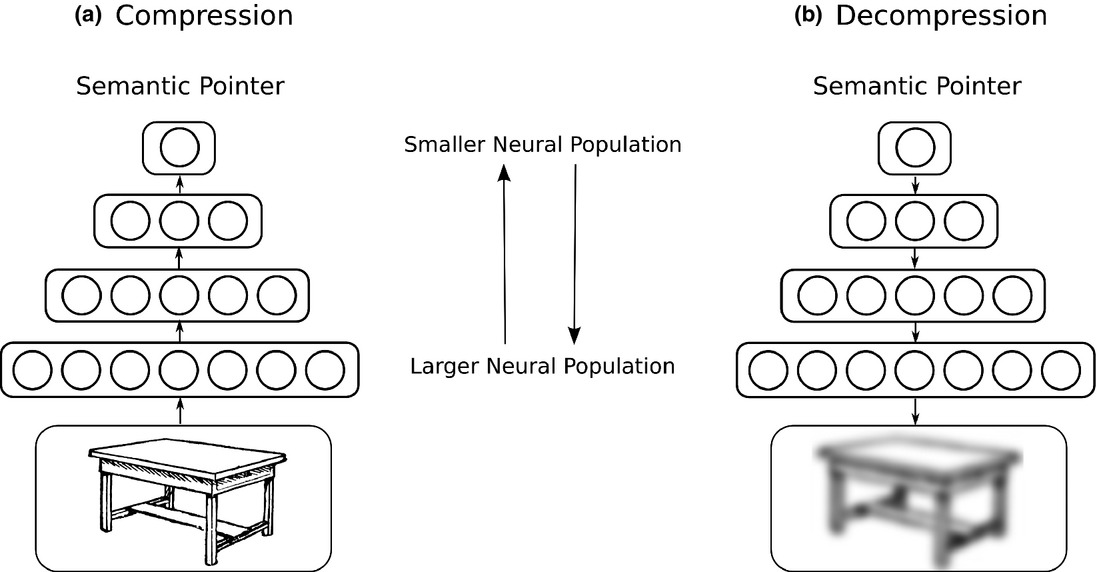
\includegraphics[width=\textwidth]{../img/semPointer.jpg}
    \caption{(a) A sensorimotor input, here a table, is compressed sequentially into a Semantic Pointer. (b) A Semantic Pointer is decompressed and returns a representation of a table. Due to the compression process the decompression results in noise. The figure is taken from Blouw et al. \cite{blouw2016concepts}.}
    \label{fig:sp}
\end{figure*}





\subsection{Concept space} \label{subsec:gaerdenfors}
\story{Properties of concepts, introducing the idea of concepetual spaces and a geometry of concept space (latent space)}

Gärdenfors offers a geometric interpretation of cognition that serves as a bridge between the sub-symbolic and the symbolic, between the perceptual and the conceptual \cite{Gaerdenfors}. Her argues that concepts can be represented as regions in a conceptual space, where the dimensions of the space correspond to the different features or properties that can be used to describe the concepts.

In this model, each quality dimension — be it temperature, weight, brightness, or hue — becomes an axis in a multi-dimensional space. Concepts are then regions within these spaces. Imagine, if you will, a three-dimensional space where color is represented: one axis for hue, another for saturation, and a third for brightness. A "concept" like 'red' would be a specific region in this 3D color space.


In mathematical terms, a set is convex if, for every pair of points within the set, the line segment connecting them is also contained within the set. Imagine a balloon. If you pick any two points within the balloon and draw a line between them, that line never leaves the space of the balloon. In Gärdenfors' geometric concept space, most concepts are "convex" regions. For example, if you have a swan and a goose and consider them both as instances of "bird", then it's likely you'll consider everything in between also a "bird".


[expound on that, and relate to rest]

% Peter Gärdenfors' theory of conceptual spaces is a geometrical framework for representing and reasoning about concepts \cite{Gaerdenfors}. Gärdenfors argues that concepts can be represented as regions in a conceptual space, where the dimensions of the space correspond to the different features or properties that can be used to describe the concepts.

% For example, the conceptual space for colors might have dimensions for brightness, saturation, and hue. The conceptual space for animals might have dimensions for size, weight, and diet.

% Gärdenfors proposes that natural concepts are typically \emph{convex}. This means that any two points in the convex region are connected by a line that lies entirely within the region.

% Gärdenfors argues that the convexity constraint is important for a number of reasons. First, it allows us to reason about the relationships between concepts in a natural way. For example, we can say that the concept "red" is more specific than the concept "color" because the convex region for red is contained within the convex region for color.

% Second, the convexity constraint allows us to model a variety of cognitive processes, such as categorization, reasoning, and analogy. For example, we can say that an object belongs to a category if it is located within the convex region for that category.

% Third, the convexity constraint is consistent with our perceptual and motor experiences. For example, the convex regions for colors correspond to the different ways in which we perceive colors.

% Gärdenfors illustrates the idea of convexity with the following example:

% Imagine a cone, where the base of the cone represents the concept "bird" and the apex of the cone represents the concept "robin." All other birds, such as penguins, eagles, and sparrows, would fall within the cone.

% This is because a robin is a more specific type of bird than any other type of bird. In other words, all robins are birds, but not all birds are robins.

% Gärdenfors argues that some concepts, such as "tall" and "short," are \emph{concave}. This means that there are two points in the convex region that are not connected by a line that lies entirely within the region.




% Conceptual spaces are a theoretical framework for understanding how humans represent and reason about concepts. The framework was developed by Peter Gärdenfors in the 1980s and 1990s, and it has been highly influential in the fields of cognitive science, cognitive linguistics, and artificial intelligence. \source[inline]{reference his book}

% Gärdenfors defines a conceptual space as a geometric space where concepts are represented as points or regions. The dimensions of the conceptual space correspond to the different features or properties that can be used to describe concepts. For example, the conceptual space for colors might have dimensions for brightness, saturation, and hue.

% The geometry of the conceptual space allows us to reason about the relationships between concepts. For example, we can define the distance between two concepts as the distance between the corresponding points or regions in the conceptual space. This allows us to measure the similarity between concepts, as well as the degree to which one concept is more specific than another.

% Gärdenfors argues that conceptual spaces provide a powerful framework for understanding how humans represent and reason about concepts because they are:

% Expressive: Conceptual spaces can be used to represent a wide range of concepts, including concrete concepts (e.g., colors, shapes), abstract concepts (e.g., love, justice), and even relationships between concepts (e.g., father-of, above).
% Natural: Conceptual spaces are grounded in our perceptual and motor experiences. For example, the dimensions of the conceptual space for colors correspond to the different ways in which we perceive colors.
% Flexible: Conceptual spaces can be used to model a variety of cognitive processes, including categorization, reasoning, and analogy.

\source[inline]{Gardenfords book (2004)}


\begin{itemize}
    \item Hyberbolic space (relate to holarchies)
\end{itemize}

I suspect that we use symmetry as an inductive bias [relate to dehaene]. The concept of opposites is a type of symmetrical relation where two entities are diametrically opposed on a spectrum or scale. Day and night, hot and cold, up and down — these pairs may help us organize our world into understandable categories. Of course there are many other types of symmetry, which could act as important inductive biases in order to construct a conceptual world model, 
\begin{description}
    \item[Reflectional Symmetry] When one half is the mirror image of the other half. E.g., many human faces or butterfly wings.
    \item[Rotational Symmetry] When an object looks the same after a certain amount of rotation. E.g., a regular pentagon or a snowflake.
    \item[Translational Symmetry] When an object can be moved (or translated) a certain distance and appear unchanged. E.g., wallpaper patterns.
    \item[Bilateral Symmetry] Seen in many animals, where the left and right halves of an organism are mirror images of each other.
    \item[Radial Symmetry] Where symmetry is centered around a central axis, like in starfish or daisies.
    \item[Spiral Symmetry] Seen in objects like shells or certain galaxies, where there's a continuous curve centered on a point.
    \item[Chiral Symmetry] Refers to objects that are mirror images but not superimposable, like left and right hands.
    \item[Time Symmetry] In physics, certain processes are time-symmetric, meaning they can proceed forward or backward in time without violating the laws of physics.
    \item[Scale Symmetry] When patterns look the same at any scale. Fractals are an example of this.
    \item[Oppositional Symmetry] In abstract terms, where concepts have opposites or counterparts, like good/evil, light/dark, or positive/negative.
\end{description} 

\improvement[inline]{isn't that already inherent since ANNs are doing linear algebra? I think the ANNs are capable of finding symmetrical relations but it could be a more explicit inductive bias/ heuristic? like we see that LLMs find some relations (man : king :: woman : queen), but it could be used explicitly for the construction of concepts. Also think about relational }
[insert figure]










\section{What is Meaning?}
- what do the symbols mean? or "what's all that jazz (for concepts or so)"




Conceptual role semantics (CRS) is the view that the meanings of expressions of a language (or other symbol system) or the contents of mental states are determined or explained by the role of the expressions or mental states in thinking. The theory can be taken to be applicable to language in the ordinary sense, to mental representations, conceived of either as symbols in a ‘language of thought’ or as mental states such as beliefs, or to certain other sorts of symbol systems. CRS rejects the competing idea that thoughts have intrinsic content that is prior to the use of concepts in thought. According to CRS, meaning and content derive from use, not the other way round.






\section{What is a thought?}
\begin{itemize}
    \item Explain the idea of a thought as a trajectory through semantic space. 
    \item How does this trajectory look like in LLMs? (Wolfram)
    \item How does this trajectory look like in GFlowNet? (perhaps operationalised as a Markovian trajectory?)
    \item How does a thought look like in enactivist/ purely reactive or reflexive cognitive frameworks. 
    \item Thought as constructing probabilistic programs
    \item What does it mean to have a model?
    \item What do we model? Res extensa, Res cogitans. The inside as well as the outside world (Reference Solms, JB, Decartes)
    \item What does it mean to compute?
    \item Can any concept be definitively defined as a particular concept (either symbolic or symbolic vector e.g. SPA, hyperdimensional vectors) or are all concepts approximations?
\end{itemize}

















\section{What Does It Mean to Understand?}
\subsubsection{Operationalising "Understanding"}
\begin{itemize}
    \item Reverse Engineering: Is understanding being able to reconstruct the thing we want to understand? If you can break down an object or concept and then reconstruct it, perhaps it implies you understand it.
    \item Modelling: Understanding might be proportional to the model we create of a concept. The more accurate and comprehensive our model, the greater our understanding.
    \item Utilization: It could also be the degree to which we can use a concept. If we can apply it effectively, we could claim to understand it.
    \item Maybe understanding is the size/ strength of a concept? Imagine it as blobs in an abstract space, a large blob with many connections would be understood, whereas a new little blob with little connections is not. 
\end{itemize}



What does it mean to truly understand something? 

I would say that understanding requires causality, not just correlation. (Searle's chinese room)

Is it possible for artificial intelligence to grasp the essence of a concept like “body” or “mass”? It can approximate to an arbitrary degree but you can't square the circle, i.e. approximations at the limit do not become the thing approximated, they are just treated as such. This is related to joscha bach's interpretation of Gödel's theorem, that it cannot be implemented since there are no infinities in physical reality. Anyways, approximations might be enough, and might be what we're doing too. This is important for the symbolic vs connectionist debate.

GPT learns through the context in which words and phrases appear, essentially creating a concept network of words. The AI analyses this abstract relational structure to generate responses. Yet, we might question whether this process equates to understanding.

The conundrum is reminiscent of the mary's room thought experiment, in which Mary, despite having all the data about colour, has never truly experienced it. If she were to experience colour one day, would she glean any new information that was not already available in the data she had studied?

The question seems to probe whether phenomenological experience can be simulated through abstract data. While it's possible to argue that a blind man will never truly see just by reading about it, we must also consider that our experiences are essentially the result of neurons firing in our brains. If we possess the necessary cognitive mechanisms, it's plausible that phenomenological experience could be replicated by alternative means.


\begin{itemize}
    \item are human's capabilities (or LLMs) just a bunch of bag of tricks, masquerading in a trenchcoat.
    \item induction, deduction, abduction, inference to the best explanation
    \item "Although it is not clearly understood by many, classic grounded theory utilizes deduction, induction, and abduction as the necessary logic functions of the research process. Glaser’s described the forms of logic—induction, abduction, and deduction—but referred to them as conceptualization, theoretical coding, and theoretical sampling. Induction begins with data and produces concepts, which are the building blocks of grounded theory. Employing abduction, the analyst infers relationships among the concepts to develop interrelated hypotheses. Deduction is used to gather data to fill in the gaps and produce an explanatory theory. Each type of logic is indispensable to classic grounded theory method. The purpose of this methodological paper is to briefly describe the process and product of each type of logic as applied to the language and procedures of classic grounded theory. - The Logic and Language of Classic Grounded Theory: Induction, Abduction, and Deduction" [is this related to the way concepts share information and are constructed? top down (deduction), bottom up (induction), lateral (abduction), maybe not because different truths are established? check this]
\end{itemize}


\subsection{Hemispheric Lateralisation}
\begin{itemize}
    \item notion that if we don't have a concept for it, it does not exist for us. I.e. even if our sensory equipment can in principle take it in, and does take it in, it is not there for us. It seems we are unable to attend to it. Perhaps attribute meaning to it and therefore it doesn't enter our conscious awareness.
\end{itemize}



\info[inline]{argument for hemispheric lateralization}
\begin{itemize}
    \item Broad vs narrow attention. One sees the trees, the other the forest.
    \item the left wants to jump to conclusions and is much more quick and dirty, while the right says hang on
    \item left deals with things that are known, when something isn't, its better to leave it to the right until it can be categorised by the left
    \item things in the left are more isolated, while in the right everything is connected to everything else
    \item left is static, right is flowing and changing
    \item the left abstracts, the left is more interested in categories, the right in the unique case
    \item the left sees things as inanimate, the right sees them as animate
    \item as we age we use the representations of what we know increasingly, neglecting the world. We become more solipsistic. This makes sense because perceiving things for the first time is computationally heavy and expensive, so the things we know from experience will usually be good enough.
    \item Talk about confabulation
\end{itemize}

Often, the most obvious things, once unpacked, reveal the most [examples?]. Our most basic perceptions and assumptions are so deeply integrated into our cognitive processes that they become invisible to us, essentially automatic. When driving the same route everyday, people may arrive at their destination without conscious awareness of it. Tasks become automated. [show studies, other examples like piano.]

From a computational standpoint, one could say that these deeply embedded perceptions function much like 'compiled code' in a computer program — efficient and fast, but not easily inspected or altered. These perceptions are model-based representations optimized for computational efficiency, trading off flexibility for speed. They exist as pre-computed "shortcuts" that enable us to interact with the world without incurring high computational costs each time we encounter a familiar situation.

In machine learning, this relates to the trade-off between model-based and model-free learning. Model-free approaches require higher computational costs upfront but are more adaptable. Model-based strategies offer efficient but rigid ways to interact with the world. Both strategies have their pros and cons, reflecting a trade-off between computational efficiency and cognitive flexibility. [source]

As we age, we rely increasingly on these internal representations instead of engaging directly with external reality, making our view of the world more solipsistic. [source]

\improvement[inline]{think of two types of intelligences (crystal vs fluid ?), also exploration exploitation}
\improvement[inline]{We can also include barbara oakley on types of focus, deep and direct, vs broad}

This phenomenon can be explained by the increasing reliance on "cached" or "memoized" cognitive models, which offer a computationally cheaper way to navigate reality. It's a form of cognitive "greedy algorithm," opting for local optimizations based on past experience rather than recalculating the optimal path each time. [source + relation to predictive coding paradigm]

This concept parallels the notion of "overfitting" in machine learning, where a model becomes so tailored to the training data that it loses generalizability. In human cognition, an over-reliance on established mental models could result in decreased adaptability and an insular worldview, effectively isolating the individual from the ever-changing external environment.

As we automate more cognitive functions—either through learned habits or technological aids—we engage less in "active sampling" of the world, reducing the richness and nuance in our perceptions. This leads to a form of "lossy compression" of reality, where only the most salient features, according to our models, are retained.


- Problems should be solved at the lowest possible level of the hierarchy. Larger goals require more sophisticated organization.
- How does a system recognize that it cannot solve it alone and that it needs to recruit other cells? Think of the computational boundary. Perhaps we must be able to estimate computational complexity. 
- This compression of sensory information into concepts may be the origin of symbolic processing. 

- Things we don't have concepts for don't exist. We can't describe them in our language. [related to joscha about truth.] 





% \section{Spaces in Cognition}
% \subsection{Latent Spaces}
% \subsection{Cognitive and Conceptual Spaces}
% \subsubsection{Peter Gärdenfors's Perspective}
% \subsection{The Geometry of Cognitive Spaces}
% \subsubsection{Hyperbolic Spaces} (aligns with holarchies)

\begin{itemize}
    \item show representations in human brains and argue why the brain may largely be a generative model. 
\end{itemize}

A paradigm, coming originally from Ethology is the idea of reactive agents which have four defined "rules" on which they act (Murphy, 2000). Reflexes are hard-wired responses to certain stimuli. Think of a knee-jerk reaction. Taxes
define the movement of an organism towards (or away from) a certain stimuli. An example is the way ants follow a trail by chemotaxis. More complex behaviour is elicited through fixed-action-patterns. These consist of a sequence of certain behaviours, usually triggered by some stimulus. A squirrel's nut burying behaviour is an example. Lastly, the sequencing of innate behaviours such as a digger wasp's brood-tending is an example of even more complex behaviour. Further, it has been shown how complex behaviour can emerge as an epiphenomenon such as in swarms, ants (Franks, 1989) or even in Conway's popular Game of Life (Conway, 1970).



\begin{itemize}
    \item Efficient inference over hierarchical Bayesian models is still difficult.
    \item Approximate inference
    \item Here we can go into models monte carlo e.g. etc.
    \item Einstein: intuition, rationality
\end{itemize}


\section{What Is a Language?}




\begin{itemize}
    \item Children use language without knowing what the words actually mean. The meaning is the context. 
    \item People can even teach without understanding. (so there seems to be a depth to understanding (maybe relate to SPA, shallow vs deep))
    \item Fake it 'til you make it?
    \item Is the limit of imitation a clone? ()
\end{itemize}






\subsection{Language in Thought}
\begin{itemize}
    \item Syntax \& Semantix
    \item Jabberwocky sentences (would be equivalent to a sentence that doesn't minimize surprise well (given the task, because it could also be a goal))
\end{itemize}

\begin{itemize}
    \item Sapir-Whorf
    \item Why do we need language
    \item Does meaning emerge in LLMs (is meaning the network or do we need grounding)
    \item Grounding
    \item Binding problem ( how do we assign meaning to geometrical features of stimuli)
    \item McLuhan.
\end{itemize}


Think about Wittgenstein and the notion that language is the limit of your reality.   
“The limits of my language mean the limits of my world.”  
“the world we see is defined and given meaning by the words we choose. In short, the world is what we make of it.”

Alfred Korzybski:
our reality is limited by the human nervous system and our language
Since we are limited by our nervous system and our language, we never have direct access to reality.
“A map is not the territory it represents, but, if correct, it has a *similar structure* to the territory, which accounts for its usefulness.”

This may relate to donald hoffman in that we have some handle on reality but it is obscured by our interface to it. 



\begin{itemize}
    \item Natural language as semiotic pointers to concepts. (think about alan moore to spell, etc. also advertisement, doublespeak, rhetoric, etc.)
    \item personality changes with language (hebrew vs german)
    \item English is an expressive language, a front-end, a communicative tool. Underneath, is a language of thought. It writes our conceptual world model. We are guided by our world-model, our ideology, our interpretation of reality and the truth and conclusions we derive from it. 

    We can speak from compassion, from hate, from jealousy, apathy, love, and so on. This is not just emotional expression but it encodes our identity, attitude, and our beliefs. 
    
    Language is symbolic, it point to concepts, and it is in the same class of concepts as money, a collective imaginary category.
    
    In order for our communication to be effective and useful, we need to create some shared framework. If we use different currencies and cannot convert between them, we cannot be in the same market. There needs to be some bridge that is accepted by both sides, so that we can interact. This is the same in language. We need to be able to translate. A translation is a mapping between two symbolic systems that point to the same concept.   
    
    If we use the same language, but change its meaning, i.e. the symbolic pointers are orthogonal to each other, we cannot communicate anymore. 
    
    A different way to think about this, is that symbolic systems, such as language, are relative and only work if we remain within the borders of the same context. Without a common frame-of-reference, language becomes meaningless. The pointers break.
    \item     
\end{itemize}




\subsubsection{Neurosymbolic AI}
[should this be in the concept section?]

Garcez et al. analyse connectivist and symbolic paradigms and find that the most effective AI would integrate these approaches \cite{garcez2020neurosymbolic}. They find that for effective learning from data, knowledge in neurosymbolic AI should be embedded into vector representations. Once networks are trained, symbols can be extracted. These symbols are not only descriptive but also operate at an optimal level of abstraction. This facilitates infinite applications with finite resources. Furthermore, this enables compositional and discrete reasoning at the symbolic layer, providing the capability to extrapolate beyond the given data distribution. Combinatorial reasoning is challenging. The combination of learning and reasoning addresses this problem by learning to reduce the number of effective combinations. 
Consider a neural network that learns certain regularities and recognizes that whenever it sees features of type A, features of type B are also present, but features of type C are not. This implicit rule can be made explicit by converting it into symbols: $\forall x A(x) \rightarrow (\exists y B(y) \land \lnot \exists z C(z))$.


\subsubsection{Formal Grammar}
\begin{itemize}
    \item Syntax vs. Semantix
    \item Semiotics
    \item We find that GPT also finds an inherent "semantic grammar" in the data. (but we do it differently)
\end{itemize}

undecidable problems:
\begin{itemize}
    \item \rephrase[inline]{Determining if a context-free grammar generates all possible strings, or if it is ambiguous.
    Given two context-free grammars, determining whether they generate the same set of strings, or whether one generates a subset of the strings generated by the other, or whether there is any string at all that both generate.}
    \item The problem of determining the Kolmogorov complexity of a string.
    \item Planning in a partially observable Markov decision process.
    \item Game of Life
    \item halting problem
    \item polymorphic typed lambda calculus (second-order lambda calculus)
\end{itemize}

% \subsection{Gödel's Incompleteness Theorem and Turing's Extensions}
% \subsection{Chomsky's Hierarchy}
% \subsection{Computational Irreducibility}
% \subsection{Constructivism}
% \subsection{Syntax vs. Semantics in Language}
% \subsection{Semiotics}
% \subsection{The Notion of a Semantic Grammar}
% Church-Turing Thesis


\section{What Is a Computation?}

\subsection{Computational Mind}
\begin{itemize}
    \item RNA computation [paper]
    \item LCL, etc.
    \item Church-Turing Thesis
    \item Difference in computation between brain (Piccinini), ANNs and symbolic processing
    \item Is computation the only way to truth (relate this to constructivism)
    \item computational irreducibility: we can use generative models as a shortcut sometimes. we can compress regularities. But Wolfram shows that sometimes that is impossible. if truth is whatever is computable, and we take note of the idea of computational irreducibility, it means that there are some computations in which we must apply every step to get there. there is no shortcut. 
\end{itemize}




\begin{itemize}
    \item Do we have one generative model or multiple competing models (multiple DSLs, trying to find the best one)? Or do we just have competing representations at the frontier and it is more difficult to change beliefs deeper in the conceptual space, where concepts are foundational and others rely on?
    \item Jerome Busemeyer uses Quantum formulations to show how we are in a super-position of beliefs until we collapse them upon evidence. 
\end{itemize}




\begin{itemize}
    \item Talk about induction, deduction, abduction and how sampling from a reward distribution is similar to abduction aka inference to the best explanation
    \item add markpoels 7 criteria 
\end{itemize}









% \section{What is a Holarchy?}




% \subsection{Part-Whole Hierarchies/ Holarchies}
% \story{we make explicit that holarchies are fundamental emergent structures and show how to build them}


% A holon has an identity and that identity can be interpreted, which creates meaning. 

% The holon transcends and includes. It is dynamic and it changes. When it changes, it changes its identity and therefore, the meaning that can be derived from it. 

% An atom, when it accepts more protons and electrons, changes its identity and function and ability to connect with other atoms.





% A holarchy is a system in which each whole is made up of parts, and each part is a whole in itself. Holarchies are nested, meaning that each whole is also a part of a larger whole. This structure is similar to a hierarchy, but with the important difference that holarchies are non-linear. In other words, there is no single top-down chain of command. Instead, each level of the holarchy is interconnected and interdependent.

% The concept of holarchy was first introduced by Ken Wilber in the 1970s [source], an extrapolation of Arthur Koestler's notion of a Holon, a thing that is simultaneously a whole and part of a larger whole, following the cybernetic tradition of studying the complex dynamics of self-organizing systems. Wilber realized that the human mind and society could also be understood as holarchies, and he developed his integral theory to describe this structure in detail.

% One of the key features of holarchies is that they are emergent. This means that the properties of a holarchy cannot be predicted by simply understanding the properties of its parts. For example, the behavior of a human brain cannot be fully explained by understanding the behavior of individual neurons. Instead, the brain's emergent properties, such as consciousness and intelligence, arise from the complex interactions of its many parts.


% \begin{itemize}
%     \item argue thoroughly why the conceptual framework is built as a holarchy
%     \item We agree on an assumption that we construct a model of the world.
%     \item What exactly would an explicit model or an implicit model or no model at all look like?
%     \item We agree that there are certain hierarchical relationships. [example book, music, ontology, etc.]
%     \item Here we can talk about conceptual structures, holarchy, part-whole hierarchies. 
%     \item How concepts are split with more attention, etc. 
%     \item Do the upper levels of a holarchy control the lower levels? I.e. Does the holarchy become a heterarchy?
%     \item Heterarchy, sand example in nested organism pregnancy friston paper, DNA, GEB
%     \item Multi-scale systems
%     \item Ontology
%     \item Mereology? and relation to Category theory?
%     \item This is essentially learning a 
%         \item hierarchical LVM
%         \item hierarchical graphical model
%         \item Parse tree
%         \item Can be formalised as Context Free Grammar. 
%         \item The grammar here is the generative model. 
%         \item What is a generative model?
%         \item A generative model is simply a probabilistic description of how causes (i.e., latent states) generate consequences (i.e., data or sensations). \cite{friston_world_2021}
%     \item Include Hofstader levels of abstraction (let's have a coffee.)
% \end{itemize}





% \subsection{Active Inference} \story{Introducing the shared principle to build multi-scale systems. Essentially a formalization of discernment. homeo-allostasis }
% \cite{Ramstead_Kirchhoff_Friston_2020}
% Ramstead et al. make the distinction between \emph{active} inference and \emph{enactive} inference. 

% "active inference," is a corollary Karl Friston's Free Energy Principle [source]. This framework posits that living systems minimize a variational free energy function to maintain themselves in a state that is compatible with their existence. Here, cognition is essentially about predictive modeling, and action is how an agent resamples the environment to minimize the error in its predictions. The agent, in this frame, is akin to a scientist, continually updating its internal models of the world to reduce surprises and fulfill its own expectations. It's a constant renegotiation of hypothesis and test, theory and experiment, query and observation.

% "Enactive inference," on the other hand, draws more from the "enactive" tradition of cognitive science, inspired by figures like Francisco Varela and Evan Thompson [source]. This perspective argues that cognition is fundamentally rooted in an organism's interactions with its environment, emphasizing a co-constitutive relationship between the two. There's a deeper focus here on the importance of embodiment and the constitutive role that action plays in shaping cognitive structures. Mind and world, subject and object, create each other in a reciprocal embrace. It's less about a model inside the head predicting the world and more about the continual creation of a world through interaction.


% \rephrase[inline]{From Maxwell Ramstead Tutorial on active inference}



% Caucheteux et al. provide evidence that the human brain continuously predicts a hierarchy of representations that spans multiple timescales and also that syntactic and semantic predictions are processed separately \cite{caucheteux_evidence_2023}. This differs from LLMs which are trained to predict the next token. [maybe put this in language section]

% The complexity of the human brain arises from its intricate structure, both in terms of its physical components and its functional organization. A comprehensive understanding of the brain requires a multilevel approach that spans from the microscopic scale of molecules to the macroscopic scale of brain systems and interactions with the environment.

% At the most foundational level, the brain's function rests on the interactions of its cellular components. Neurons, the primary cellular units of the brain, are responsible for processing and transmitting information. These transmission processes are facilitated by neurotransmitters, the chemicals that help propagate signals across synapses, the specialized junctions between neurons.

% Beyond individual neurons, the microcircuit level involves small neural networks. These are clusters of interconnected neurons that serve specific functions. Whether it's processing particular sensory information or executing a distinct motor task, these microcircuits play a pivotal role in the brain's operational hierarchy.

% Scaling upwards, the brain is segmented into specific brain areas and nuclei, each playing a unique functional role. For instance, the hippocampus is crucial for memory processes, while the basal ganglia are deeply involved in movement and motor coordination.

% At the systems level, individual brain areas are not isolated entities but are part of broader brain systems. These systems, such as the limbic system responsible for emotion and motivation, comprise various interrelated structures, e.g., the amygdala, hippocampus, and certain sections of the thalamus.

[is this section too long? maybe shorten it, we get it, the brain is a hierarchy..]
 

% At the pinnacle of brain organization, we find the integration of all its parts. The brain's two hemispheres, the left and right, offer different functional specialties. For instance, in a majority of right-handed individuals, language processing predominantly occurs in the left hemisphere [go into McGilchrist hemisphere differences? or in sys1,2, section?]. Furthermore, the integration of the brain and spinal cord establishes the central nervous system, crucial for sensory information relay and motor command execution.

% The brain does not function in isolation. It's in a continuous dialogue with the body and the external environment. The brain-body interaction underlines the significance of feedback loops that shape brain processes. Simultaneously, social and environmental interactions influence the brain, underscoring the interdependence between an individual and their surroundings.

\cite{Park_Friston_2013}
One can witness that the brain, in its form and function, encapsulates a hierarchy that reflects the multifaceted layers of its surroundings. A paper by Park \& Friston goes further to demonstrate that the brain showcases nested networks that include structures as micro as dendrites to as macro as entire brain regions.

These multi-scale systems operate not only in the spatial dimension, from microcosm to macrocosm, but also temporally. They span across phylogenetic, epigenetic, and ontogenetic timescales. This poses a challenge: how can we address these diverse spatial and temporal scales in a principled manner? What framework can effectively encompass this vast range of scales?

Most natural systems that are self-organizing tend to dissipate, as highlighted by Vernon [reference]. They increase entropy, which in this context, can be perceived as a measure of potential configurations a system could inhabit. A system with high entropy has a myriad of configurations available, while one with low entropy has limited options.

Surprisingly, about 80\% of the brain's connections are involved in feedback [source, predictive coding]. Such a significant portion of the brain's energy is invested in a system that seems to serve a feedback purpose. 

% The predictive processing paradigm posits that instead of viewing the brain as a passive data collector, the brain is a query mechanism, primarily engaged in top-down prediction. The primary function becomes producing predictions about imminent sensory inputs. What ascends is the prediction error, the mismatch between predictions and actual sensory input. In this framework, perception becomes an inquiry-response mechanism, much like a Google search. The brain, through active inference, seeks to reverse the causality arrow, shifting from received data to inferring the probable causal factors. 

% This continuous feedback mechanism constantly compares expectations with actual perceptions. To minimize discrepancies, the brain can either modify its model or alter its environment. How do we quantify the effectiveness of such a model? 

A common approach involves constructing various models encoding diverse hypotheses and evaluating their ability to account for data variance. Condensing this process yields the concept of *variational free energy*. Crucially, it's not analogous to thermodynamic energy; it gauges how efficiently a model explains data variance.

The term 'variational free energy' draws parallels with thermodynamics. In thermodynamics, free energy represents the residual energy in a system capable of work. In information theory, it denotes the remaining room for parameter adjustments.

The concept of the Markov blanket suggests that given a set of states, the sensory and active states of a system remain independent of external world states. Active inference narrates how internal (model-encoding) and active (akin to skeletal muscles) states adapt to minimize free energy, enabling inference.

Every component in this complex system is itself a system, from entire organisms to individual cells. Each component, being Markov-blanketed, can infer its position relative to others, provided communication exists. By sharing a generative model, units at one level can enact target morphologies.






\subsection{Self-organization and predictive processing} \cite{friston_world_2021}
As the brain develops, its neurons self-organize into networks that are able to generate and test predictions about the world. This process of self-organization allows the brain to develop a model of the world that it can use to make inferences about sensory input.

One way to think about the relationship between self-organization and predictive processing is to consider how self-organization may allow the brain to develop a model of the world. As the brain develops, its neurons self-organize into networks that are able to represent different aspects of the world. For example, some networks may represent the visual world, while others may represent the auditory world or the somatosensory world.

These networks are constantly interacting with each other, and this interaction allows the brain to develop a unified model of the world. This model of the world can then be used to generate predictions about sensory input.

The identity of a multi-scale system can be thought of as the emergent properties that arise from the interactions of the different levels of organization. For example, the identity of a cell is not simply the sum of the identities of its individual molecules. Rather, the cell's identity is emergent from the way in which the molecules interact with each other to form complex structures and networks. [relate to levins part]

This is reminiscient of embedding spaces in which words are self-organizing by getting input from the world. 
\info[inline]{LLMs also create a generative model, but lack the causal structure.}




\begin{itemize}
    \item Discernment of Concepts
    \item Discernment as the primary operator. 
    \item Me against the World
    \item Homeostasis
    \item Allostasis
    \item Operational Closure
    \item Organizational Closure
    \item Intentional Stance
    \item Active inference
    \item Explain Bayes theorem and how it relates 
\end{itemize}





% active inference, effective action


% Friston et al. define \emph{free energy} as a functional of two quantities \cite{friston_world_2021}. This variational density is posited to be encoded—or parameterized—by internal states of a system. In this framework, perception equates to modulating internal states to reduce the divergence between the variational and the posterior densities over these latent states, conditioned on observed data. Action, in contrast, changes how data or sensations are acquired, aligning them with the generative model of the agent. In sum, free energy is optimised by action and perception by maximizing a variational bound on marginal likelihood.



% The authors define three unknowns, which need to be optimized, corresponding to the generative model: 
% \begin{enumerate}
%     \item the latent states that generate the outcomes
%     \item the model parameters that encode the statistical regularities of the model
%     \item the architecture of the model itself
% \end{enumerate}
% [refer to this in the PPL section]

% Each of these latents is accompanied by a variational density or Bayesian belief, parameterized by an agent's states, weights, and structural elements. 

% Friston highlights the importance of the representation of uncertainty when abiding by the free-energy principle, namely that we must optimize posterior probabilities - point estimates are not sufficient. [refer to this when discussing MLE over MAP] This makes the problem inherently more challenging than simply computing averages or expectations.

% In computational terms, log model evidence can be dissected into accuracy and complexity components [see formula], the latter of which relates to the Kullback-Leibler divergence between the posterior and prior distributions, effectively the degrees of freedom, necessary to account for the observations [too much here?]. This exerts a simplifying pressure on the model selection, resonating with Occam's Razor [reference, glossary?] paradigms in algorithmic complexity and minimum description length [reference to MDL from dehaene et al ].

% In practice, discrete actions invoke sensory outcomes that shape approximate posterior beliefs, refined through minimizing variational free energy under probable policies. These beliefs, in turn, provide the groundwork for formulating subsequent actions. This gives rise to a self-referential cycle where agents not only predict but also validate their own behavior through sensory feedback. [maybe reference back from GFNs, when constructing policies?]


% [explain the idea of Markov blanket, etc.]






\begin{enumerate}
    % \item Constructing a conceptual framework, with relationships of all concepts.
    % \item Navigating this conceptual framework. 
    % \item maybe the generative model is correlational, while the inference model turns that into causality. (see beyond the fep internalism externalism, ramstead)
    \item I think having a sense of self, i.e. a self-referential story, involves this inference model that builds causal structure, a narrative (see \cite{bouizegarene_narrative_2020}).
    \item Is this related to interpolation vs extrapolation? (is it the same in high dimensions? chollet? lecun?)
\end{enumerate}










\improvement[inline]{this subsection has to be unpacked.}
The idea that the thoughts are constructed by some kind of Language of Thought (LOT), in order to understand and represent our reality has a long history. 
Gottfried Leibniz imagined a \textit{Characteristica Universalis}, a formal language capable of expressing metaphysical concepts \cite{sep-leibniz-logic-influence}.
Jerry Fodor, among many other scholars, continued the development of this hypothesis and proposed that our cognitive processes are akin to computations involving a system of mental representations that can be composed into complex thoughts, akin to how sentences are formed from words according to the rules of grammar \cite{sep-language-thought}. Fodor's theory implies an innate structure underlying human cognition, with systematic, rule-governed operations that manipulate symbols.


If our thoughts are indeed composed by some language, we can let our intuitions about its structure and limitations be guided by the advances made in the past century in regards to formal languages and computationalism.
Gödel showed that any formal system strong enough to express Peano Arithmetic is incomplete \cite{sep-goedel-incompleteness}. Turing showed that any possible computation can be done by a Turing machine and concluded that the human mind must be computational \cite{JCopeland2004-JCOTET}. [Piccinini disagrees]
Chomsky's Hierarchy classifies formal languages of different strengths and the automata that recognize them \cite{chomsky1959certain}.
These results and many more are consequential when thinking about a language of thought.
Many important questions about concepts are still left unanswered, e.g. regarding their formation, the structure of the framework they reside in, their representation, how they connect to other concepts and so on. 
Many contemporary versions of the LOT hypothesis (LOTH) argue that our conceptual framework is constructed bottom-up using some initial primitives. More so, the language we construct concepts in is executable, akin to a programming language \cite{dehaene_symbols_2022}. The idea is that we model the world by creating programs that generate our observations \cite{rule_child_2020}. 
Roumi et al.'s experiment indeed suggest that humans may interpret and compress sequence regularities in a type of program of minimum description length (MDL) \cite{al_roumi_mental_2021}.
Dehaene et al. further test this hypothesis and find similar results \cite{dehaene_symbols_2022}.
The question then remains, where primitives actually come from.
Piantadosi asserts that symbols have no inherent meaning, instead, meaning emerges from the dynamic relations between symbols. I.e., only the conceptual role and the dynamics of the symbols define meaning \cite{piantadosi2021computational}.
By defining meaning as an emergent phenomenon of conceptual roles, Piantadosi and Hill do not rule out that large language models (LLM) already have some foundation of meaningful concepts \cite{piantasodi2022meaning}.
Recent work tries to relate these ideas to biological systems, e.g. Quan et al. propose how role-filler interactions could be implemented in the brain via temporal synchrony to permit symbolic processing and dynamic binding of variables \cite{do2021neural}.
Santoro et al. argue for a semiotic approach, assert that symbols are subjective, and propose that meaning of symbols in artificial systems will arise when they are subjected to socio-cultural interactions \cite{santoro2021symbolic}.

Ellis et al. use $\lambda$-calculus, which is Turing complete, to build something akin to a LOT \cite{ellis_dreamcoder_2021}. In response, Piantadosi shows that combinatorial logic is equivalent to $\lambda$-calculus and why combinatorial-logic-like (LCL) language is preferable, for one because it doesn't assume primitives, thereby avoiding the problem of their meaning and origin. 
One of the questions regarding a LOT is whether thoughts can be produced by simple syntactic symbol manipulation.
I (and many others) suspect that semantics are not just an emergent phenomenon but that it actively shapes our perception and concept formation \cite{santoro2021symbolic, hofstadter_gdel_1979}.
Moreover, purely symbolic attempts, albeit being the original approach of artificial intelligence, have proven to be insufficient \cite{garcez2020neurosymbolic}. Instead, the successes of modern AI are owed to the advances of connectionist models. These however, have their own deficits, namely, being incredibly data-hungry, lacking causality, and lacking out-of-distribution generalization, to name a few. Therefore, new approaches try to combine these two AI strands into what is known as \emph{neurosymbolic AI} \cite{garcez2020neurosymbolic}.

\begin{itemize}
    \item Relation to self-organization, active inference, FEP, autopoiesis, etc. 
    \item what is a symbol and what is a symbolic architecture. symbolic here literally means symbol manipulation. context free grammar, etc. logical predicates. DC makes it neurosymbolic by using nns. I make it even more connectionist by embedding the symbols.
    \item Explain the different gradients of symbols. e.g. SPA is symbol-like. Part whole hierarchies and capsules are also kind of a symbol in that there is a central representation of a concept. I think its about centrality vs distributed representation and also about the capabilities of the symbols, i.e. does cognition work by only manipulating the symbols, rather that the representations themselves? What is that extra layer needed for then? Think of SPAs layered vectors, shallow vs deep understanding.
    \item If we argue that the LOT is a kind of a self-organising system, then what are the parts (the primitives) we construct (analogy to primes and how every natural number can be constructed using primes.) What are the primitives here? Do we have some axioms of ontology? Are they built in? I.e. taking the stance that we do not start off with a clean slate (Turing) (inductive biases?). Perhaps through evolution? 
    \item Maybe talk about the idea that concepts might start off simple, i.e. starting with light and dark, warm and cold, then increasing the complexity of concepts, like Hubel \& Wiesel. 
    \item This kinda goes back that every sacchade is a query to the world. Werner Heisenberg “What we observe is not nature herself, but nature exposed to our method of questioning.” 
    \item Relate to poverty of the stimulus
    \item relate to piaget 
    \item model vs model free (we dont just learn chess by watching, we either learn about or try to infer the rules.)
\end{itemize}

Free will: if i can out model you, i.e. i can predict every action you do (we can try this with simple organisms.)


\subsubsection{Poverty of the Stimulus}
- arg for LOT

The "poverty of the stimulus" argument is an argument that is often made in the field of linguistics and cognitive science. It argues that children are able to learn language despite being exposed to a relatively limited amount of data, which suggests that they must have some innate knowledge or ability that helps them learn language.

The argument is based on the observation that the linguistic input that children receive is often incomplete, ambiguous, or inconsistent. For example, children may hear sentences that contain errors or that are not grammatical. Despite this, children are able to learn the rules of their language and use them to produce and understand sentences that they have never heard before.


